%=========================================================

% Here you can choose to compile with or without solutions.
% However, this definition is ignored if you use any
% command from the `Makefile`.
\providecommand{\withSol}{\iftrue}

%=========================================================

\documentclass
[twoside,english,colorbacktitle,accentcolor=tud9c]
{tudexercise}

\usepackage[T1]{fontenc}
\usepackage[latin9]{inputenc}
\usepackage{amstext}
\usepackage{amsmath}
\usepackage{graphicx}
\usepackage{setspace}
\usepackage{multicol}
\usepackage{mathtools}
\usepackage{dsfont}
\usepackage{units}
\usepackage{subfigure}
\usepackage{color}
\usepackage{booktabs}
\usepackage{fancyref}
\usepackage{listings}
\usepackage[ngerman,english]{babel}

%=========================================================

\def\homework{4}
\def\homeworkVer{1}
\def\homeworkSolVer{1}
\def\lecture{Robot Learning}
\def\semester{Winter Semester 2017/2018}
\def\prof{Prof. Dr. J. Peters, D. Tanneberg, M. Ewerton}
\def\deadline{Due date: Wednesday, 31 January 2018 (before the lecture)}



%=========================================================

\ifcsname withSol\endcsname\else
  \expandafter\let\csname withSol\expandafter\endcsname
                  \csname iffalse\endcsname
\fi

\withSol
	\usepackage[solutions]{iasHomework}
\else
	\usepackage{iasHomework}
\fi


\definecolor{mygreen}{rgb}{0,0.6,0}
\definecolor{mygray}{rgb}{0.5,0.5,0.5}
\definecolor{mymauve}{rgb}{0.58,0,0.82}

\lstset{ %
	backgroundcolor=\color{white},   % choose the background color; you must add \usepackage{color} or \usepackage{xcolor}; should come as last argument
	basicstyle=\footnotesize,        % the size of the fonts that are used for the code
	breakatwhitespace=false,         % sets if automatic breaks should only happen at whitespace
	breaklines=true,                 % sets automatic line breaking
	captionpos=b,                    % sets the caption-position to bottom
	commentstyle=\color{mygreen},    % comment style
	deletekeywords={...},            % if you want to delete keywords from the given language
	escapeinside={\%*}{*)},          % if you want to add LaTeX within your code
	extendedchars=true,              % lets you use non-ASCII characters; for 8-bits encodings only, does not work with UTF-8
	frame=single,                      % adds a frame around the code
	keepspaces=true,                 % keeps spaces in text, useful for keeping indentation of code (possibly needs columns=flexible)
	keywordstyle=\color{blue},       % keyword style
	language=Python,                 % the language of the code
	morekeywords={*,...},            % if you want to add more keywords to the set
	numbers=left,                    % where to put the line-numbers; possible values are (none, left, right)
	numbersep=5pt,                   % how far the line-numbers are from the code
	numberstyle=\tiny\color{mygray}, % the style that is used for the line-numbers
	rulecolor=\color{black},         % if not set, the frame-color may be changed on line-breaks within not-black text (e.g. comments (green here))
	showspaces=false,                % show spaces everywhere adding particular underscores; it overrides 'showstringspaces'
	showstringspaces=false,          % underline spaces within strings only
	showtabs=false,                  % show tabs within strings adding particular underscores
	stepnumber=2,                    % the step between two line-numbers. If it's 1, each line will be numbered
	stringstyle=\color{mymauve},     % string literal style
	tabsize=2,                     % sets default tabsize to 2 spaces
	title=\lstname                   % show the filename of files included with \lstinputlisting; also try caption instead of title
}
%=========================================================


\newcommand{\studentdata}{Markus Lamprecht, 2424163 \qquad Moritz Knaust, 2430801}

\begin{document}
	
	\hwtitle{}
	\maketitle
	
	\begin{examheader}
		\normalsize
		\vspace{-1em}
		Name, Surname, ID Number \hfill \studentdata{}
		\vspace{-1em}
	\end{examheader} 
	
	\textbf{Name, Surname, ID Number \hfill \studentdata{}}
	
	\newif\ifvimbug
\vimbugfalse

\ifvimbug
\begin{document}
\fi

\exercise{Expectation-Maximization}

In this exercise your task is to control a 2-DoF planar robot to throw a ball at a specific target. You will use an episodic setup, where you first specify the parameters of the policy, evaluate them on the simulated system, and obtain a reward. The robot will be controlled with the Dynamic Motor Primitives (DMPs).
The goal state of the DMPs is pre-specified and the weights of the DMP
$\theta_i, i = 1 \ldots 10$ are the open parameters of the control policy. Each DoF of the robot is controlled with a DMP with five basis functions. The ball is mounted at the end-effector of the robot and gets automatically released at time step $t_{\textrm{rel}}$.
We define a stochastic distribution $\pi(\vec{\theta}|\vec{\omega}) =
\mathcal{N}(\vec{\theta}|\vec{\mu},\boldsymbol{\Sigma})$, with $\vec{\omega} = \{\vec{\mu},\boldsymbol{\Sigma} \}$. \\
Your task it to update the parameters $\vec{\omega}$ of the policy using EM to maximize the expected return. In this exercises we will not
modify the low-level control policy (the DMPs) of the robot. 

A template for the simulation of the 2-DoF planar robot and plotting functions can be found at the course website. For the programming exercises, attach snippets of your code.

\begin{questions}


\begin{question}{Analytical Derivation}{5}

Using the weighted ML estimate,
\begin{equation}
    \vec{\omega}_{k+1} = \underset{\vec \omega}{\arg\max} \{ \sum_i w^{[i]} \log \pi(\vec{\theta}^{[i]};\vec{\omega})\},
\end{equation}
derive analytically the update rule for our policy $\pi(\vec{\theta}|\vec{\omega})$ for the mean $\vec{\mu}$. Show your derivations.

\begin{answer}
\begin{equation}
	\frac{\partial \vec{w}_{k+1}}{\partial \vec{\mu}} = 0
\end{equation}

\begin{equation}
 \pi (\theta^{[i]}; w) = N(\vec{\theta}|\vec{\mu},\boldsymbol{\Sigma}) = \frac{1}{\sqrt{(2\pi)^k |\boldsymbol{\Sigma}|}} exp(-\frac{1}{2} (\vec{\mu}-\vec{\theta})^T\boldsymbol{\Sigma}^{-1}(\vec{\mu}-\vec{\theta}))
\end{equation}

\begin{equation}
log(\pi (\theta^{[i]}; w)) = -log(\sqrt{(2\pi)^k|\boldsymbol{\Sigma}| })-\frac{1}{2} (\vec{\mu}-\vec{\theta})^T\boldsymbol{\Sigma}^{-1}(\vec{\mu}-\vec{\theta})
\end{equation}

\begin{equation}
\frac{\partial}{\partial \vec{\mu}}log(\pi (\theta^{[i]}; w)) = -\frac{1}{2}(2 \boldsymbol{\Sigma}^{-1} \vec{\mu} -2\boldsymbol{\Sigma}^{-1} \vec{\theta})
\end{equation}


\begin{equation}
\frac{\partial \vec{w}_{k+1}}{\partial \vec{\mu}} = 0 \rightarrow \sum_i w^{[i]} \boldsymbol{\Sigma}^{-1} {\mu}_i = \sum_i w^{[i]} \boldsymbol{\Sigma}^{-1} \theta_i \rightarrow \mu_i = \frac {\sum_i w^{[i]} \theta_i}{\sum_i w^{[i]}}
\end{equation}

\end{answer}

\end{question}

%----------------------------------------------


\begin{question}{Programming Exercise}{15}
Implement the EM algorithm using the provided framework. Your goal is to throw the ball at $\vec x = [2,1]m$ at time $t=100$. Use the weighted Maximum Likelihood (ML) solutions for updating the parameters of the policy. For the mean, use the equation derived at the previous exercise. For the covariance, the update rule is 
\begin{equation}
	\vec \Sigma_\mathrm{new} = \frac{\sum_i w^{[i]} (\vec{\theta}^{[i]}-\vec{\mu}_{\mathrm{new}})     (\vec{\theta}^{[i]}-\vec{\mu}_{\mathrm{new}})^T}{\sum_i w^{[i]}}.
\end{equation}
To calculate the weights $\vec{w}_i$ for each sample, transform the returned rewards by 
\begin{equation}
	\vec w^{[i]} = \exp ( ( \vec{R}^{[i]}(\vec{\theta}) - \max(\vec{R}) ) \beta )
\end{equation}
and normalize them, where the vector $\vec R\in \mathbb{R}^{N \times 1}$ is constructed from the rewards of the $N$ samples. The
parameter $\beta$ is set to
\begin{equation}
	\beta = \frac{\lambda}{ \max(\vec{R}) - \min(\vec{R}) },
\end{equation}
where $\lambda = 7$. Start with the initial policy 
\begin{equation}
	\pi(\vec{\theta}|\vec{\omega}) = \mathcal{N}(\vec{\theta}|\vec{0}, 10^6  \vec{I})
\end{equation}
and calculate the average reward at each iteration. Iterate until convergence or for a maximum number of 100 iterations.
We assume that convergence is achieved when the average return does not change much at every iteration, i.e., 
$$ | <\vec{R}_{i-1}> - <\vec{R}_\textrm{i}> | < 10^{-3}, $$
where $<\cdot>$ denotes the average operator.
At each iteration use 
$ N = 25 $ samples. In order to avoid getting stuck to a local optimum, we force the algorithm to explore a bit more by adding a regularization factor to the covariance of the policy,
\begin{equation}
    \vec{\Sigma}_\mathrm{new}^\mathrm{'} = \vec{\Sigma}_\mathrm{new} + \vec{I}.
\end{equation}
What is the average return of the final policy? 
Use \texttt{animate\_fig} from \texttt{Pend2dBallThrowDMP.py} to show how the final policy of the robot looks like (attach all five screenshots).

\begin{answer}
Average Return of the final policy: -38.89
\begin{center}
	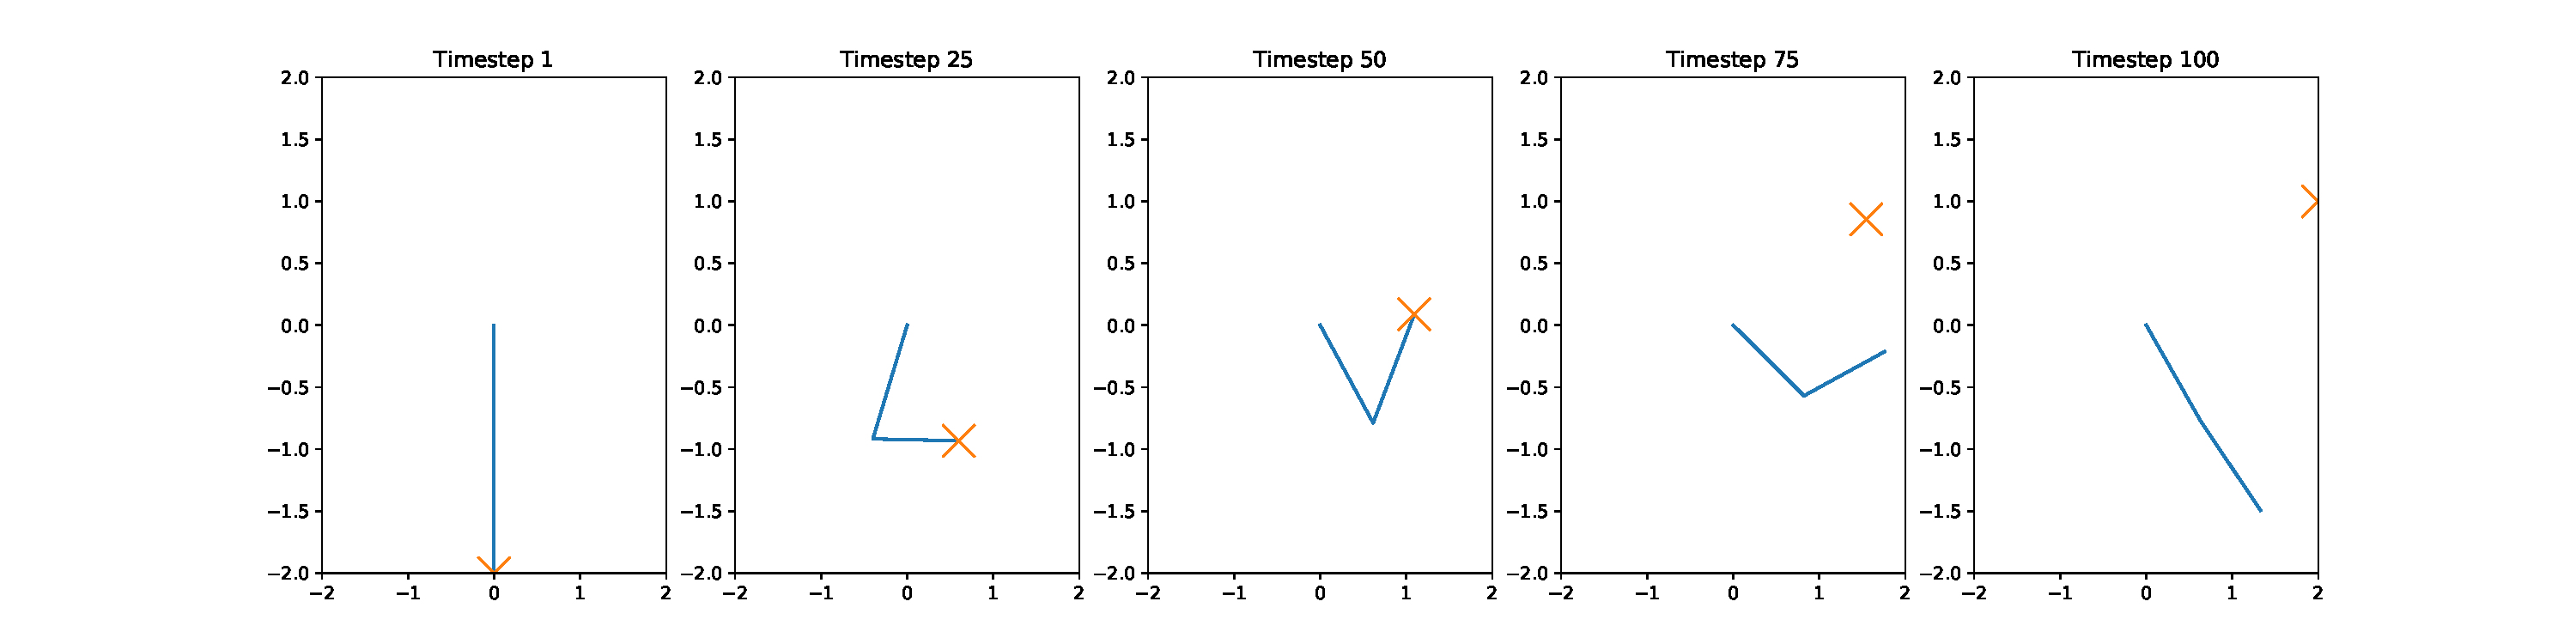
\includegraphics[width=1\textwidth]{img/EM-b.pdf}
	\captionof{figure}{Policy of the Robot's arm (blue) and the Ball's position (yellow cross)}
\end{center}
\lstinputlisting[caption=EM algorithm]{code_text/1b.py}
\end{answer}

\end{question}


%----------------------------------------------

\begin{question}{Tuning The Temperature}{5}
Repeat the learning 10 times and plot the mean of the average return of all runs with $95\%$ confidence for temperatures $\lambda = 25$, $\lambda = 7$ and $\lambda = 3$. How does the value of $\lambda$ affect the convergence of the algorithm in theory and what do you observe in the results? 
Use the logarithmic scale for your plot.

\begin{answer}
In the results we observe, that for $\lambda=25$ the average return converges faster than for smaller lambdas. Moreover it should be noted that for $\lambda=7$ we have the smallest average return at episode=100.\\

In Theory: With the temperature $\lambda$ one can select how the maximum of the weights is selected:
\begin{equation}
	\lim_{\lambda \rightarrow \infty} w^{[i]}: \text{weights are selected deteministically}
\end{equation}

\begin{equation}
\lim_{\lambda \rightarrow 0} w^{[i]}: \text{weights are selected stochastically}
\end{equation}

In the plots we can prove that for small lambdas the convergence is slower because the weights are selected stochastically. However the mean of the average reward for the last episode should be the smallest if the lambda is very small. This theoretical fact differs from the plot above.
\end{answer}

\begin{center}
	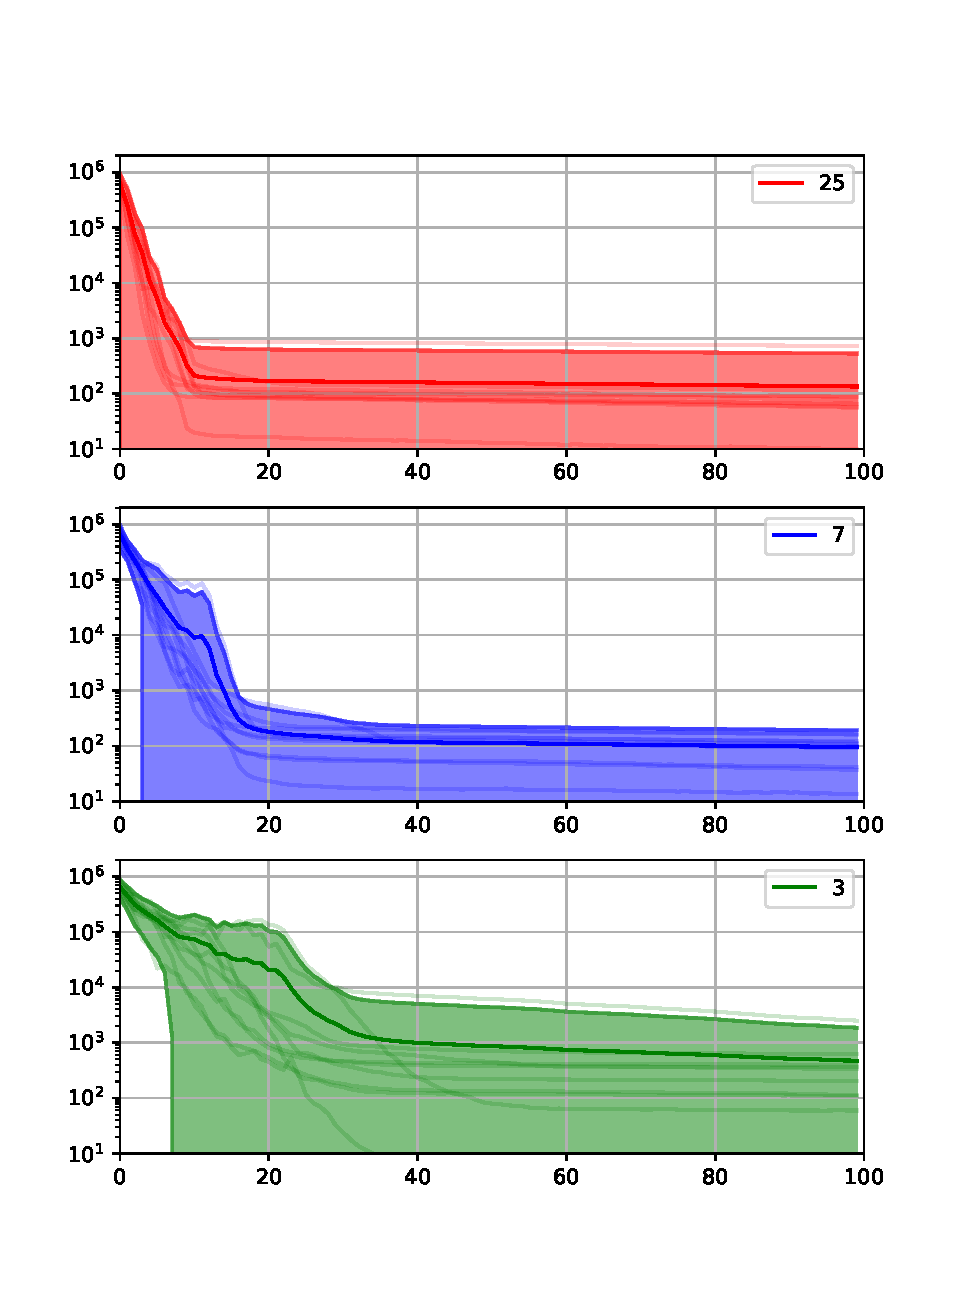
\includegraphics[width=0.5\textwidth]{img/EM-c.pdf}
	\captionof{figure}{The average return of different $\lambda$ over the episodes of the EM-Algorithm. }
\end{center}

\end{question}

%----------------------------------------------

\begin{question}[bonus]{Optimal Temperature}{5}
The problem of choosing $\lambda$ falls under a more general RL problem. Which one?
Which algorithm would allow you to automatically select the optimal $\lambda$? Explain it with your words.
Does it still have hyperparameters to be set?

\begin{answer}
RL problem: Policy Search Methods using Policy Gradients finding the right weights scaling factor. 
\\
 Algorithm that selects automatically the right lambda: Reward Weighted Regression.

The Reward Weighted Regression\\ is an algorithm that generalizes the EM algorithm. This algorithm reduces the problem of learning with immediate rewards to a reward-weighted regression problem with an adaptive, integrated reward transformation for faster convergence.  The resulting algorithm is efficient, learns smoothly without
dangerous jumps in solution space, and works well in applications of complex high degreeof-freedom robots.

Hyperparameters:\\
A transformed Hyperparameter still has to be set in RWR. However this parameter is automatically updated. With this parameter the convergence speed can be selected.
\end{answer}


\end{question}


\end{questions}


	
	\exercise{Policy Gradient}
In this exercise, you are going to solve the same task of the previous exercise but using policy gradient. 
For the programming exercises, you are allowed to reuse part of the EM code. 
Attach snippets of your code.

\begin{questions}

%----------------------------------------------

\begin{question}{Analytical Derivation}{5}
 	You have a Gaussian policy with diagonal covariance, i.e., $\pi(\vec \theta | \vec \omega) = \gauss{\vec \mu}{ \diag(\vec \sigma^2)}$, where $\vec \omega = [\vec \mu,\vec \sigma]$.
 	Compute analytically the gradient of the logarithm of the policy with respect to the parameters $\vec\omega$, i.e., $\nabla_{\vec\omega} \log \pi(\vec \theta | \vec \omega)$. (Hint: consider the properties of the diagonal covariance matrix.)
\begin{answer}
	 		
	 		\begin{equation}
	 		\nabla_{\vec\omega} \log \pi(\vec \theta | \vec \omega) = \nabla_{\vec\omega} (-log(\sqrt{(2\pi)^k} |diag(\sigma^2)|)-\frac{1}{2} (\theta-\mu)^T diag(\sigma^2)^{-1} (\theta-\mu) )
	 		\end{equation}
	 		
	\begin{equation}
	\nabla_{\vec\omega} \log \pi(\vec \theta | \vec \omega) = \nabla_{\vec\omega} (-log(\sqrt{(2\pi)^k} (\sigma^{2k}))-\frac{1}{2 \sigma^2} \sum_{i=1}^k (\theta_i - \mu_i)^2)
	\end{equation}
	
\begin{equation}
\nabla_{\vec\omega} \log \pi(\vec \theta | \vec \omega) = \begin{bmatrix}
\frac{\partial}{\partial \mu}\log \pi(\vec \theta | \vec \omega)\\\frac{\partial}{\partial \sigma}\log \pi(\vec \theta | \vec \omega)
\end{bmatrix}
\end{equation}

\begin{equation}
\frac{\partial}{\partial \mu}\log \pi(\vec \theta | \vec \omega)=\frac{1}{\sigma^2} \sum_{i=1}^{k}(\theta_i - \mu_i)
\end{equation}

\begin{equation}
\frac{\partial}{\partial \sigma}\log \pi(\vec \theta | \vec \omega)=-\frac{2k}{\sigma}+\frac{1}{\sigma^3} \sum_{i=1}^{k}(\theta_i - \mu_i)^2
\end{equation}

Note that:
 	 		\begin{equation}
 	 		\gauss{\vec \mu}{ \diag(\vec \sigma^2)}=\frac{1}{\sqrt{(2\pi)^k} |diag(\sigma^2)|} exp(-0.5 (\theta-\mu)^T diag(\sigma^2)^{-1} (\theta-\mu))
 	 		\end{equation}	 	
 		
 	\begin{equation}
(\theta-\mu)^T diag(\sigma^2)^{-1} (\theta-\mu) = \frac{1}{\sigma^2} \sum_{i=1}^k (\theta_i - \mu_i)^2
  \end{equation}

	\end{answer}

\end{question}

%----------------------------------------------

\begin{question}{Programming Exercise}{5}
	Consider the same robotic task as in the previous exercise and this time solve it with policy gradient. 
	Use an initial mean of $\vec \mu_0 = [0 \dots 0]$ and a fixed $\vec \sigma = \diag([10 \dots 10])$ (i.e., do \textbf{not} update $\vec\sigma$). Set the learning rate to $\alpha=0.1$ and use the same hyperparameters as before (25 episodes sampled for each iteration and max 100 iterations).\\
	Repeat the learning 10 times and plot the mean of the average return of all runs with $95\%$ confidence.
	Use the logarithmic scale for your plot. Comment your results.
	
	\begin{answer}
	\begin{equation}
		\omega_{k+1}=\omega_k + \alpha \nabla_{\omega} J_{\omega}
	\end{equation}
Update rule for $\theta$:
		\begin{equation}
		\sigma_{k+1}=\sigma_k + \alpha \frac{\partial}{\partial \sigma} J({\sigma_k})
		\end{equation}
		
		Update rule for $\mu$:
		\begin{equation}
		\mu_{k+1}=\mu_k + \alpha \frac{\partial}{\partial \mu}  J({\mu_k})
		\end{equation}



TODO PLOT HERE
	\end{answer}
\end{question}


%----------------------------------------------


\begin{question}{A Little Trick}{5}
	How would you improve the above implementation? (Beside using a smaller or adaptive learning rate, or using the natural gradient). What is the theory behind this ``trick''? Repeat the learning and discuss the results.
	
	\begin{answer}
	\begin{equation}
	\nabla_\omega J_\omega \sum_{i=1}^{N} \nabla_\omega log \pi (\theta; \omega)(R_i - b)
	\end{equation}
		
	The baseline has to be subtracted. Thereby the possibly high gradient of the variance can be reduced. It is still unbiased.
	
	\begin{center}
		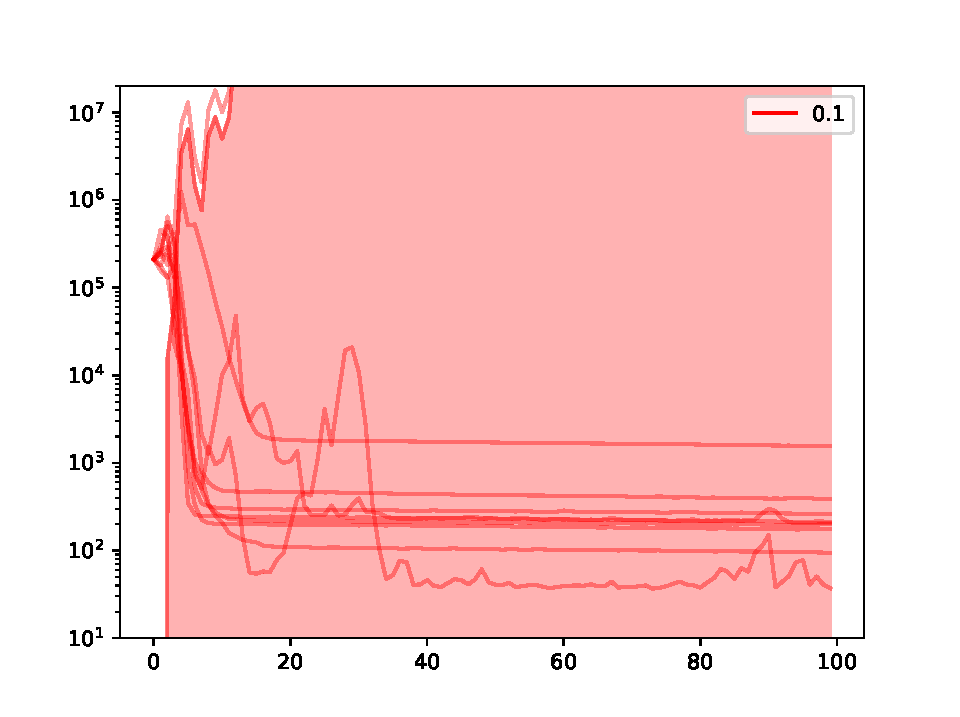
\includegraphics[width=0.5\textwidth]{img/PG-c.pdf}
		\captionof{figure}{The average return over the episodes of for $\lambda=0.1$ with baseline subtracted of the PG algorithm}
	\end{center}
	
	\end{answer}

\end{question}
	

%----------------------------------------------

\begin{question}{Learning Rate}{5}
	Repeat the optimization changing the learning rate to $\alpha=0.4$ and $\alpha = 0.2$ (keep the trick of the previous exercise).
	Plot in one figure the mean of the average returns for all $\alpha$ with $95\%$ confidence.
	How does the value of $\alpha$ affect the convergence of the algorithm? 
	Use the logarithmic scale for your plot.
		
\begin{answer}
The higher the $\alpha$ the faster the algorithm converges.

	\begin{center}
		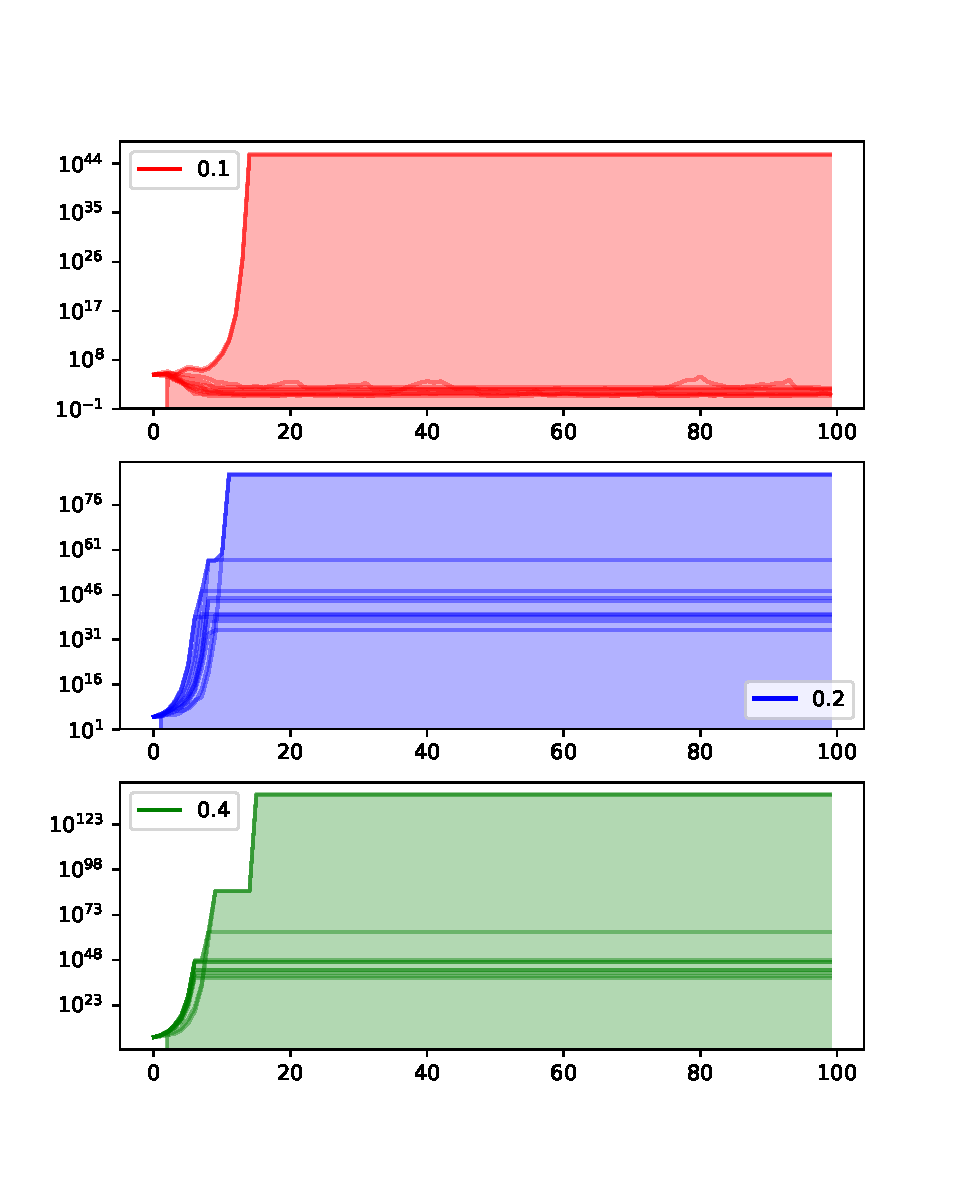
\includegraphics[width=0.5\textwidth]{img/PG-d.pdf}
		\captionof{figure}{The average return over the episodes for different learning rates $\alpha$ }
	\end{center}
\end{answer}
\end{question}

%----------------------------------------------
	
\begin{question}{Variable Variance}{5}
	Try to improve the optimization process by learning also the variance $\vec \sigma$. Is it easier or harder to learn also the variance? Why?
	\\Without using the natural gradient, tune the learning process to \textbf{achieve better results}. If you think it is necessary, you can impose a lower bound to avoid that the variance collapses to infinitely small values (e.g., if $\sigma(i)<\sigma_{\text{lower}}$ then $\sigma(i) = \sigma_{\text{lower}}$).
	In one figure, plot the learning trend with confidence interval as done before and compare it to the one achieved with $\alpha = 0.4$ before.
	
\begin{answer}
	Now use:
\begin{equation}
\sigma_{k+1}=\sigma_k + \alpha \frac{\partial}{\partial \omega} J({\sigma_k})
\end{equation}
% Füge update rule für sigma ein.
\end{answer}

\end{question}

%----------------------------------------------

	
\begin{question}[bonus]{Natural Gradient}{5}
	Write down the equation of the natural gradient. What is the theory behind it?
	Is it always easy to use?
	
\begin{answer}
The Natural Gradient: (with G the Fischer Information Matrix)
\begin{equation}
	\nabla_\omega J = G(\omega)^{-1} \nabla_\omega J
\end{equation}
Theory of the Natural Gradient:\\
KL divergence is a measure of how close a distribution is to another distribution.This brings us to the natural gradient. If we blindly update our network in the direction of its gradients, there are no guarantees the distribution of the new network will be similar to the old one.

To fix this, we first consider all combinations of parameters that result in a new network a constant KL divergence away from the old network. This constant value can be viewed as the step size or learning rate. Out of all these possible combinations, we choose the one that minimizes our loss function.

Basically, we're adding in a constraint to our update, that the new network will behave relatively similar to our old one. Our step size corresponds directly to the actual distribution of the network, not it's parameter's values.

This comes with the added benefit of a more stable learning process. Especially when we're updating using a randomly sampled batch, some outliers may make drastic changes to a network's parameters. With natural gradient descent, a single update can't make too much of an impact. 
	
Note that: Replacing a sigmoid activation with a tanh function would change the standard gradient, but not the natural gradient. 

Is it always easy to use:
No actually NG is much more computationally expensive compared to the simple gradient. Moreover there are two types of KL:
\begin{itemize}
	\item Moment projection
	\item Information projection (is not unique selects the mode!)
\end{itemize}

It is not so easy to select which KL should be used.

Note that KL can be approximated by the FIM which captures information how the single parameters influence the distribution.


\end{answer}
\end{question}

\end{questions}
	
	\exercise{Reinforcement Learning}

\begin{questions}
	
%----------------------------------------------

\begin{question}{RL Exploration Strategies}{10}
	In which spaces can you perform exploration in RL? Discuss the two  exploration strategies applicable to RL.
	
	\begin{answer}

	\end{answer}
\end{question}


%----------------------------------------------


\end{questions}
	
\end{document}
